\section{Ermitteln der Einfügungsdämpfung} \label{sec:umsetzung}
In diesem Kapitel wird ausführlich beschrieben, wie aus den gegebenen Gleich- und Gegentaktschaltung (siehe Anhang Aufgabenstellung) die Einfügungsdämpfung ermittelt wird. Um die einzelnen Schritte konsistent zu beschriebenen, wird an den entsprechenden Stellen Bezug auf die theoretischen Grundlagen Kapitel \ref{sec:Grundlagen} genommen. Der erste Abschnitt behandelt die Gleichtaktschaltung \ref{subsec:zusammenfassungGleichtakt} und in einem zweiten Abschnitt wird die Gegentaktschaltung \ref{subsec:zusammenfassungGegentakt} behandelt. In diesen beiden Kapitel wird beschrieben, wie aus den Schaltungen aus der Aufgabenstellung die Kettenmatrizen der beiden Schaltungen ermittelt wird. Aus der Kettenmatrix kann somit die Einfügungsdämpfung berechnet werden, wie in Kapitel \ref{subsec:subsec:einfuge} beschrieben.


\subsection{Gleichtaktschaltung}\label{subsec:zusammenfassungGleichtakt}
Um die Einfügungsdämpfung zu ermitteln, wird im ersten Schritt die Schaltung weitgehend vereinfacht. Die reduzierte Schaltung wird anhand der Kettenmatrix (siehe \ref{subsec:Kettenmatrix}) beschrieben. Aus der Kettenmatrix wird dann für den vorgegebenen Frequenzbereich die Einfügungsdämpung berechnet.

\paragraph{Reduktion der Schaltung}\label{para:redukGleichtakt}
Abbildung \ref{fig:CMSchaltungOriginal} zeigt die Schaltung aus der Aufgabenstellung. 
\begin{figure}[H]
	\centering
	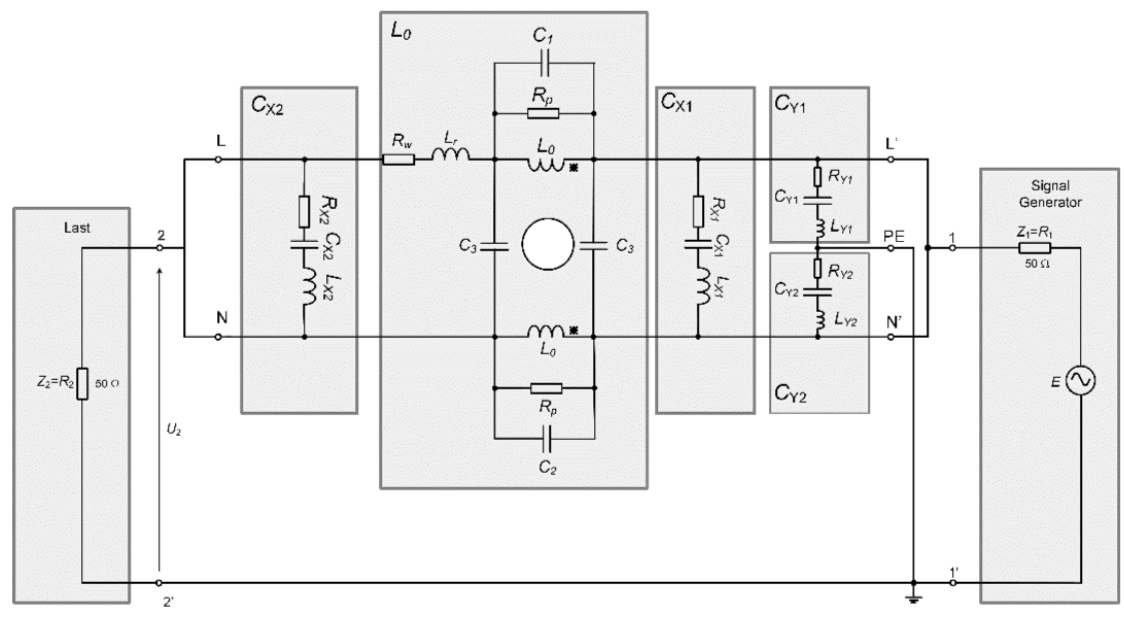
\includegraphics[width = 15cm]{CM_Aufgabenstellung.png}
	\caption{Originale Gleichtaktschaltung\cite{aufgabenstellung}}
	\label{fig:CMSchaltungOriginal}
\end{figure}
Die Originalschaltung wird mit den Komponenten $R_w$ und $L_r$ ergänzt, sodass sie symmetrisch ist. Dies macht es möglich, dass die Schaltung weiter vereinfacht werden kann. Zudem wurden $C_1$ und $C_2$ in $C_p$ und $C'_p$ umbenannt um zu zeigen, dass es sich um die gleiche Kapazität handelt. Durch weglassen des Eisenkerns, wird $L_0$ und $L'_0$ mit dem Vorfaktor zwei ergänzt da sich die Magnetfelder überlagern. %TODO besser schreiben%
Durch diese Änderungen ergibt sich die Schaltung in Abbildung \ref{fig:CMSchaltungErgänzt}.
\begin{figure}[H]
	\centering
	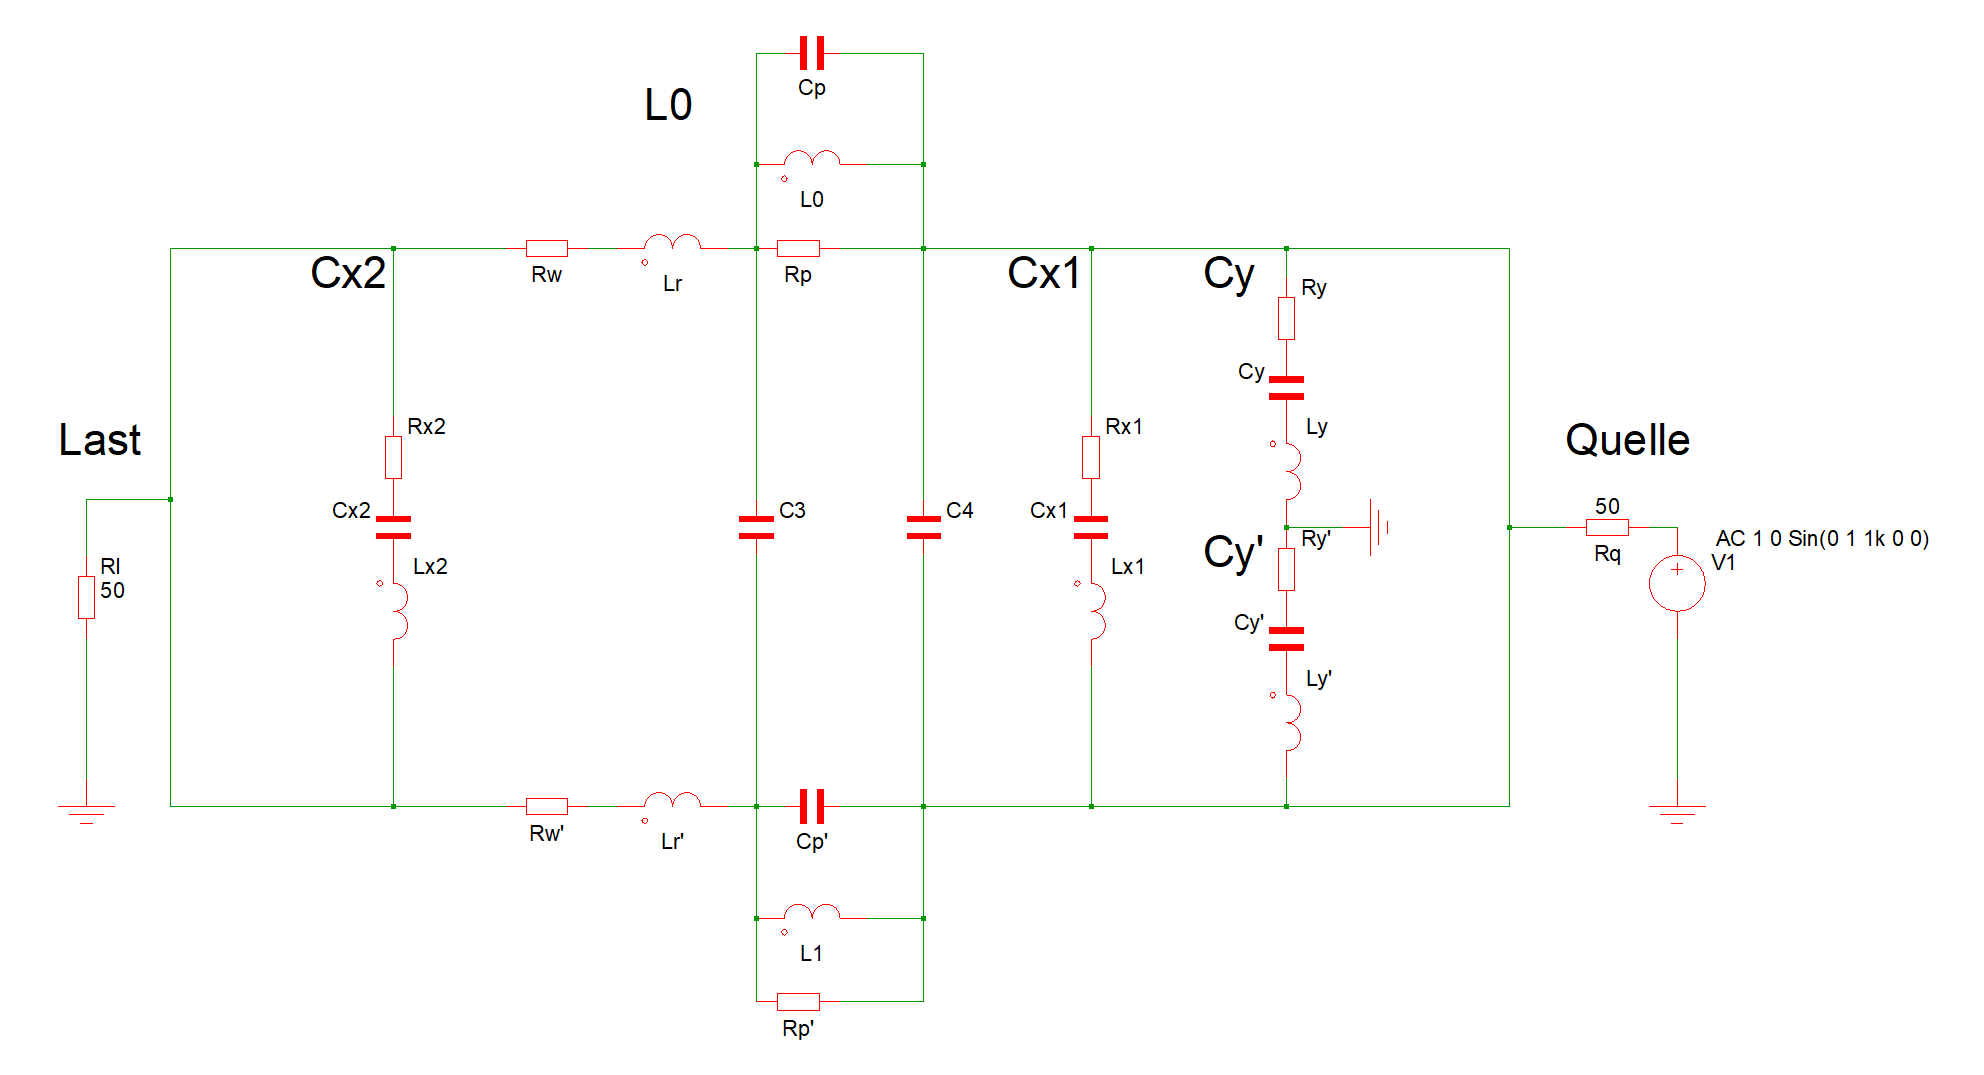
\includegraphics[width = 15cm]{EMI_CMpretty1.png}
	\caption{Ergänzte Gleichtaktschaltung}
	\label{fig:CMSchaltungErgänzt}
\end{figure}
 Der obere Strang(siehe Abbildung \ref{fig:CMSchaltungErgänzt}, Nr. 1) und untere Strang (siehe Abbildung \ref{fig:CMSchaltungErgänzt}, Nr. 2) sind identisch. Da es keinen Potentialunterschied zwischen ihnen gibt, kann die Schaltung entlang der Symmetrie-Achse (siehe Abbildung \ref{fig:CMSchaltungErgänzt}, Nr. 3) aufgetrennt werden. Dies ergibt die Schaltung in Abbildung \ref{fig:CMSchaltungaufgetrennt}.

\begin{figure}[H]
	\centering
	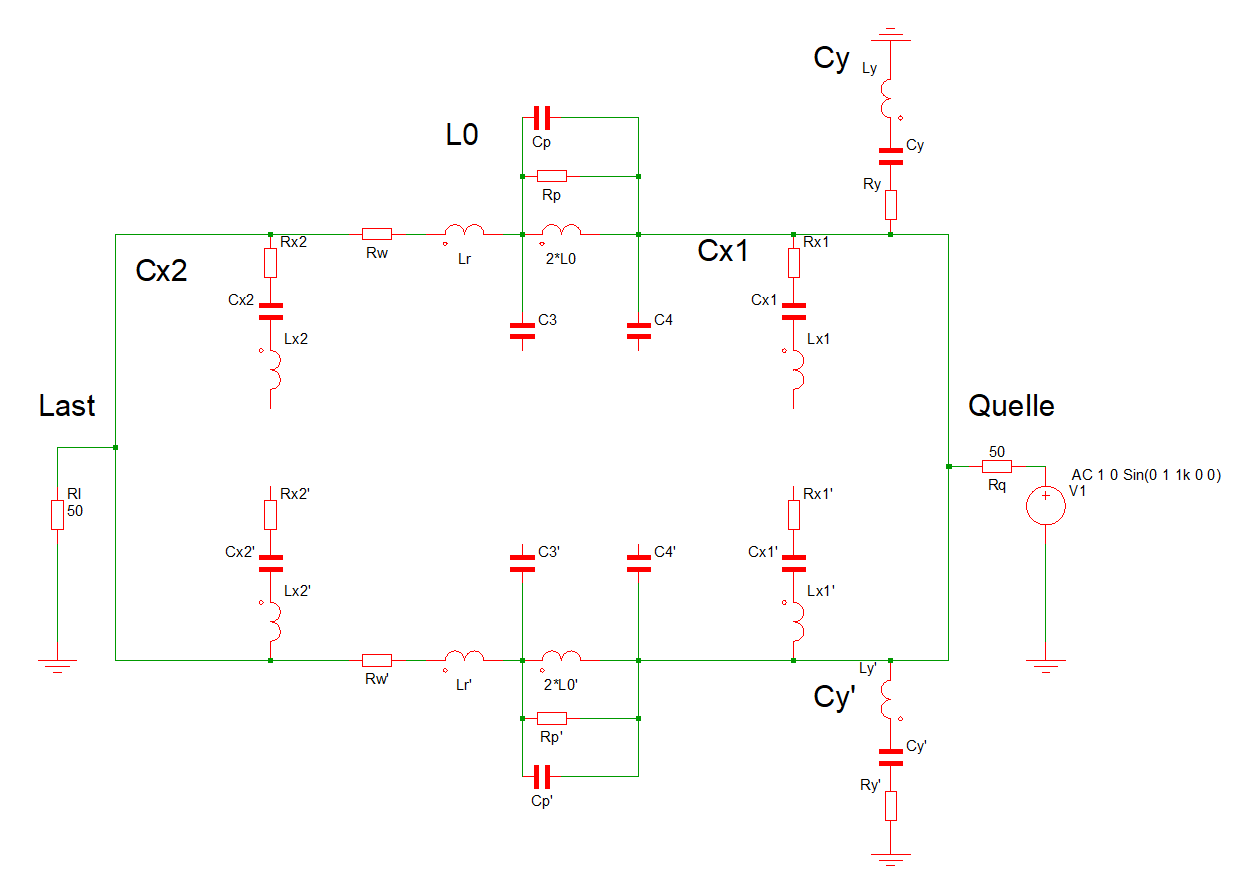
\includegraphics[width = 15cm]{EMI_CMpretty2.png}
	\caption{Aufgetrennte Gleichtaktschaltung}
	\label{fig:CMSchaltungaufgetrennt}
\end{figure}
Komponenten die nicht mehr fest verbunden sind, fallen weg. Dies gilt für die Kondensatoren $C_3$, $C_4$, $C_{x1}$ und $C_{x2}$. Die weiter reduzierte Schaltung wird in Abbildung \ref{fig:CMSchaltungvereinfacht1} abgebildet.
\begin{figure}[H]
	\centering
	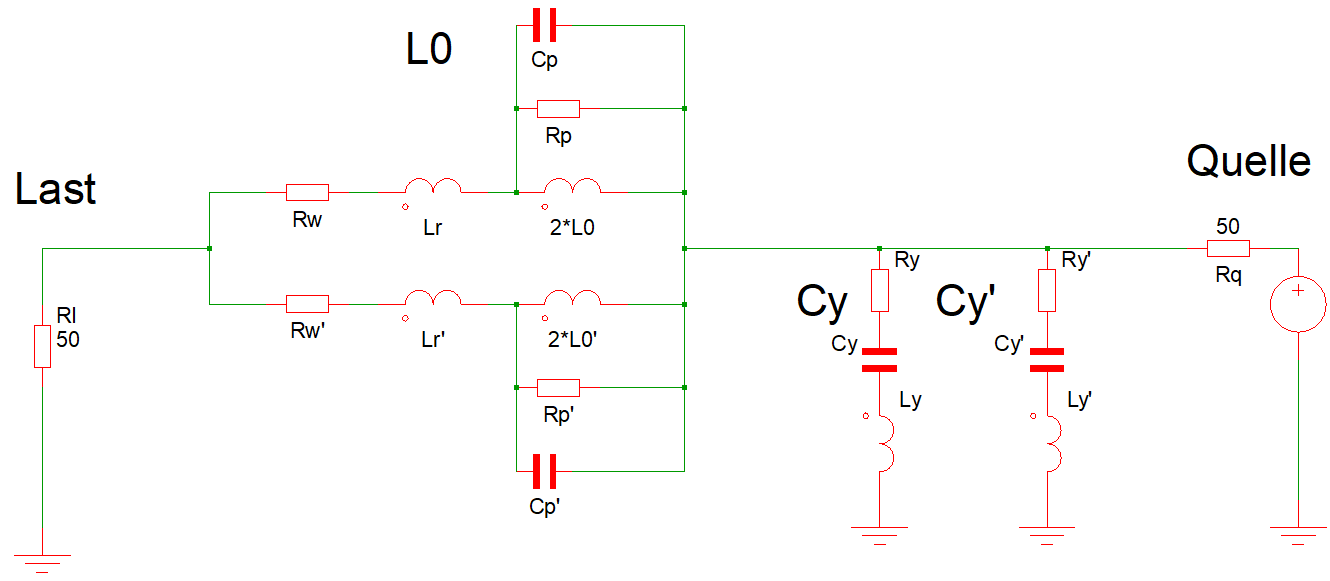
\includegraphics[width = 15cm]{EMI_CMpretty3.png}
	\caption{Vereinfachte Gleichtaktschaltung}
	\label{fig:CMSchaltungvereinfacht1}
\end{figure}
Die übrigen Komponenten von $L_0$ bilden eine Parallelschaltung, welche sich durch halbieren der Widerstände und Induktivitäten und verdoppeln der Kapazitäten zusammenfassen lässt. Zusätzlich werden die beiden $C_y$ und $C'_{y}$ parallel auf das Bezugspotential geschalten. Da $C_y$ und $C'_y$ identisch sind, werden sie wie in Abbildung \ref{fig:CMSchaltungvereinfacht} zusammengefasst. Diese vereinfachte Schaltung bildet die Grundlage für die Berechnungen der Software.

\begin{figure}[H]
	\centering
	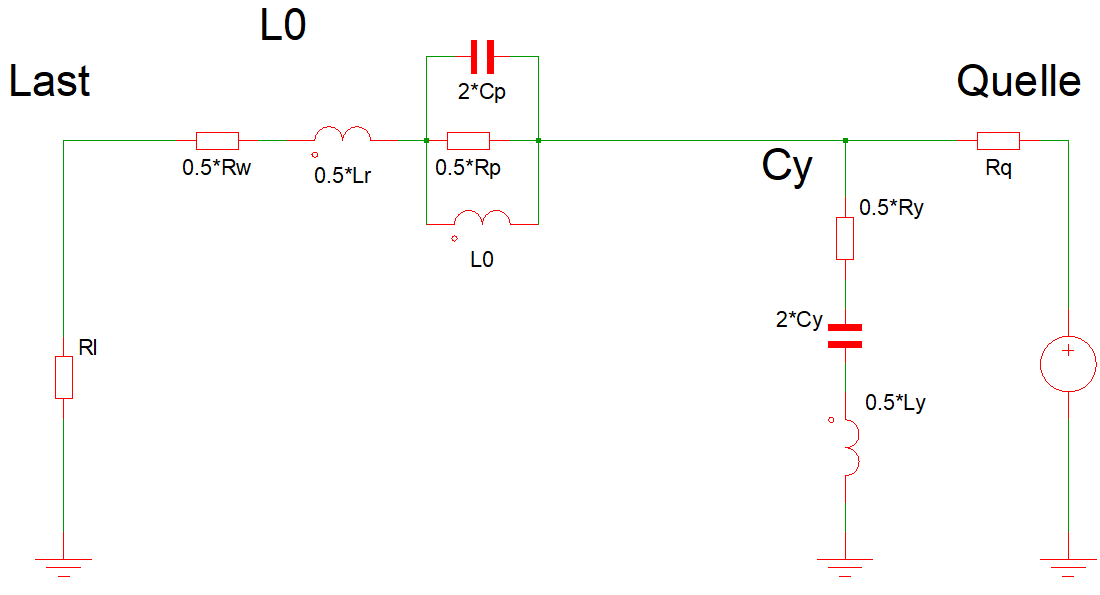
\includegraphics[width = 15cm]{EMI_CMpretty.png}
	\caption{komplett reduzierte Gleichtaktschaltung}
	\label{fig:CMSchaltungvereinfacht}
\end{figure}

\paragraph{Bilden der Kettenmatrix}\label{para:kettenGleichtakt}
Damit die Kettenmatrix der Gesamtschaltung gebildet werden kann, wird in einem ersten Schritt die reduzierte Schaltung in Längs- und Querimpedanzen (siehe Kapitel \ref{subsec:kettenmatrix}) eingeteilt. Diese werden in Abbildung \ref{fig:cmschaltungEingeteilt} mit den Kennzeichnungen „QI“ und „LI“ vermerkt wobei „QI“ für Querimpedanz steht und „LI“ für Längsimpedanz. Die Impedanzen der einzelnen Schaltungsteile werden in die Kettenmatrizen für Quer- und Längsimpedanz eingesetzt. Die Kettenmatrizen werden durch Kaskadierung zur Kettenmatrix der Gesamtschaltung zusammengefasst.
\begin{figure}[H]
		\centering
		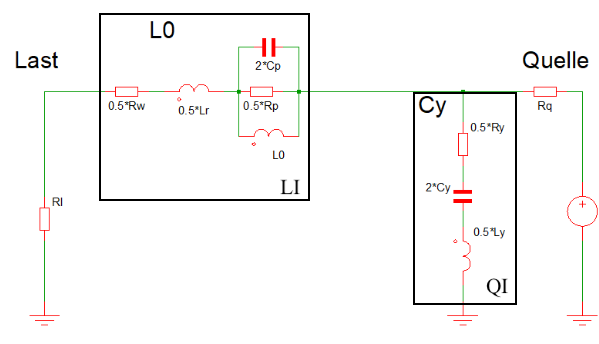
\includegraphics[width = 15cm]{EMI_CMvereinfacht_markiert.png}
		\label{fig:cmschaltungEingeteilt}
		\caption{Einteilung der Gleichtaktschaltungteile}
\end{figure}
Anhand der Kettenmatrix der Gesamtschaltung kann die Einfügungsdämpfung direkt ermittelt werden gemäss Kapitel \ref{subsubsec:streuparameter}. 

\subsection{Gegentaktschaltung}\label{subsec:zusammenfassungGegentakt}
\paragraph{Reduktion der Schaltung}\label{para:redukGegentakt}
Folgender Abschnitt legt Schritt für Schritt dar, wie die Gegentaktschaltung vereinfacht wird. Die Abbildung \ref{fig:DMSchaltungAufgabenstellung} zeigt die Originalschaltung, wie Sie der Aufgabenstellung entnommen wurde. In einem ersten Schritt wird die gekoppelte Spule (Im Bild L0) vereinfacht. Die Magnetfelder der beiden Induktivitäten L0 kompensieren sich gegenseitig. Sie fallen weg, da sie Niederohmig werden. Somit verschwindet L0 mit den parasitären Elementen C1, C2 und die beiden Widerstände Rp.
\begin{figure}[H]
	\centering
	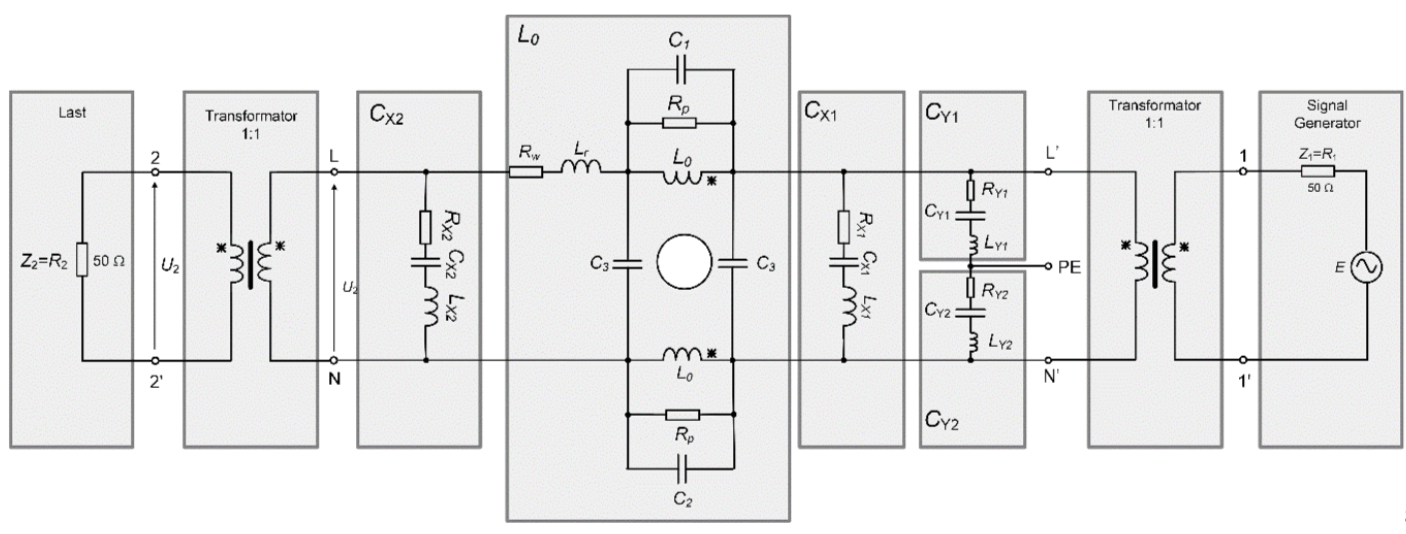
\includegraphics[width = 15cm]{DM_Aufgabenstellung.png}
	\caption{Originale Gegentaktschaltung}
	\label{fig:DMSchaltungAufgabenstellung}
\end{figure}
Durch diese Veränderungen erhält man die Gegentaktschaltung mit reduziertem L0(Abbildung \ref{fig:DMSchaltungreduziertL0}). Damit die Symmetrie der Schaltung gegeben ist, werden im unteren Strang Rw’ und Lw’ ergänzt. Diese Änderungen sind auch in der Gleichtaktschaltung vorhanden. Zudem werden die Kondensatoren C3 und C4 entfernt. Die Einflüsse sind aufgrund der kleinen Kapazität zu vernachlässigen. 
\begin{figure}[H]
	\centering
	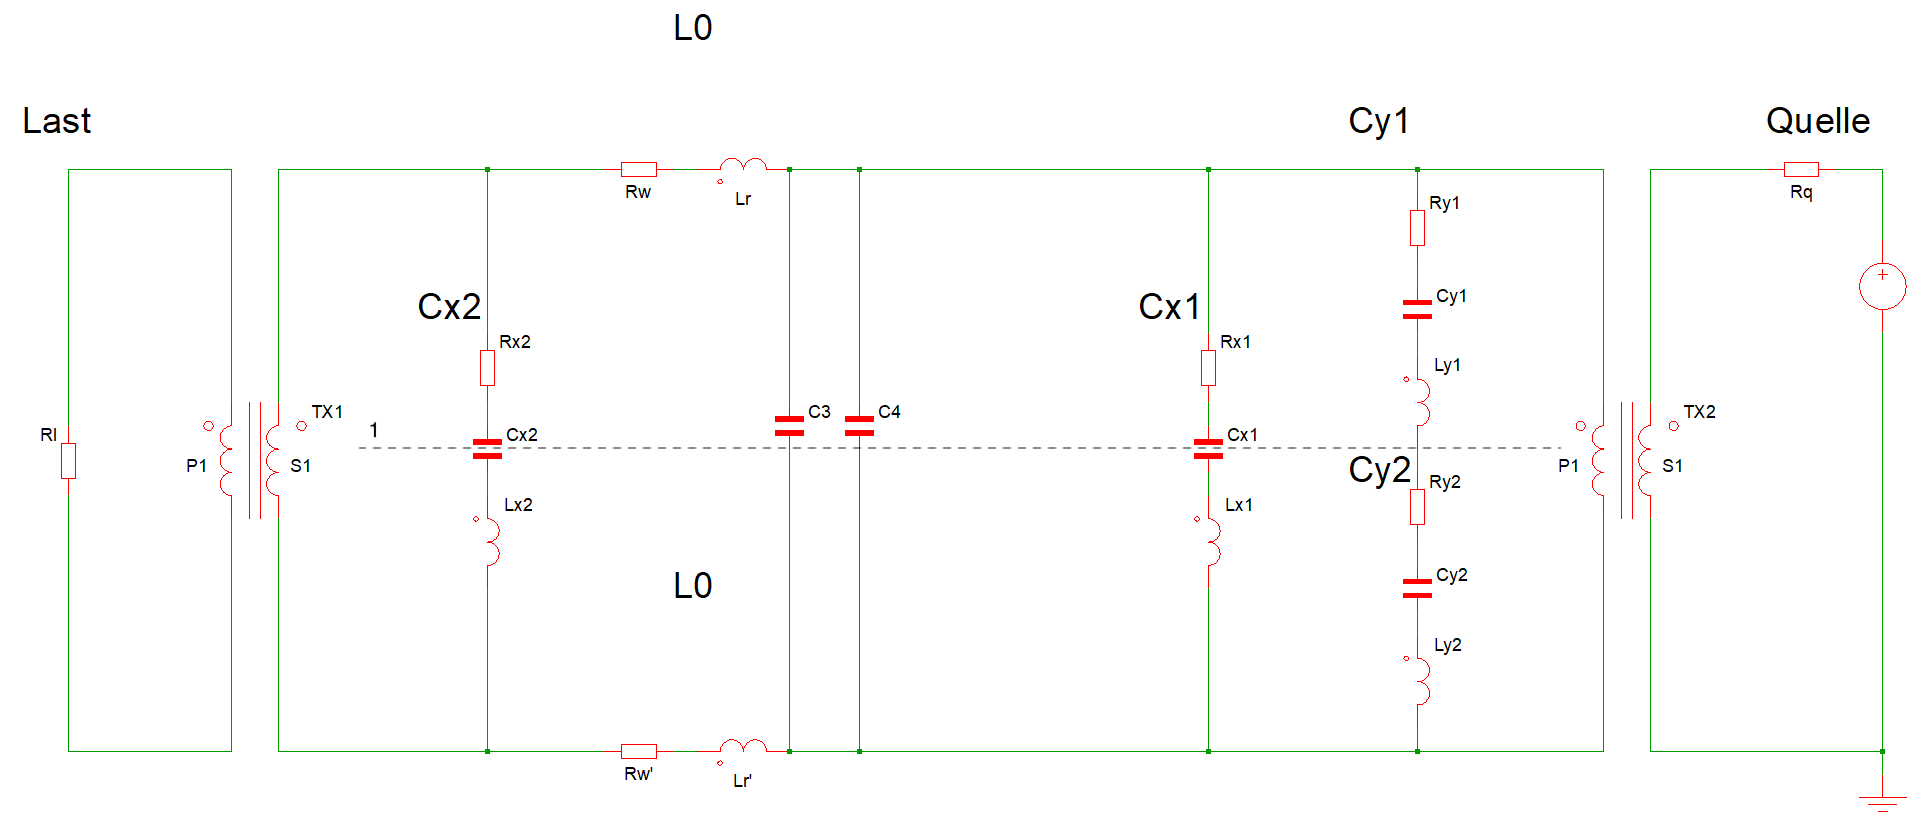
\includegraphics[width = 15cm]{EMI_DMpretty4.png}
	\caption{Gegentaktschaltung mit reduziertem L0}
	\label{fig:DMSchaltungreduziertL0}
\end{figure}
In einem nächsten Schritt wird mithilfe der Symmetrie der Schaltung weitere Teile zusammengefasst. Die im Bild eingezeichnete Linie(Abbildung \ref{fig:DMSchaltungreduziertL0}, Nr.1) entspricht der Symmetrie. Entlang dieser Linie werden die Verbindungen getrennt. Die offenen Enden werden auf das Bezugspotential geschalten. Dabei werden bei den aufgetrennten Verbindungen die elektrischen Komponenten aufgeteilt. Widerstände und Induktivitäten werden halbiert und die Kapazitäten verdoppelt. Durch dieses Vorgehen ergibt sich die Schaltung, wie in Abbildung \ref{fig:DMSchaltungSymAufgetrennt} ersichtlich.
\begin{figure}[H]
	\centering
	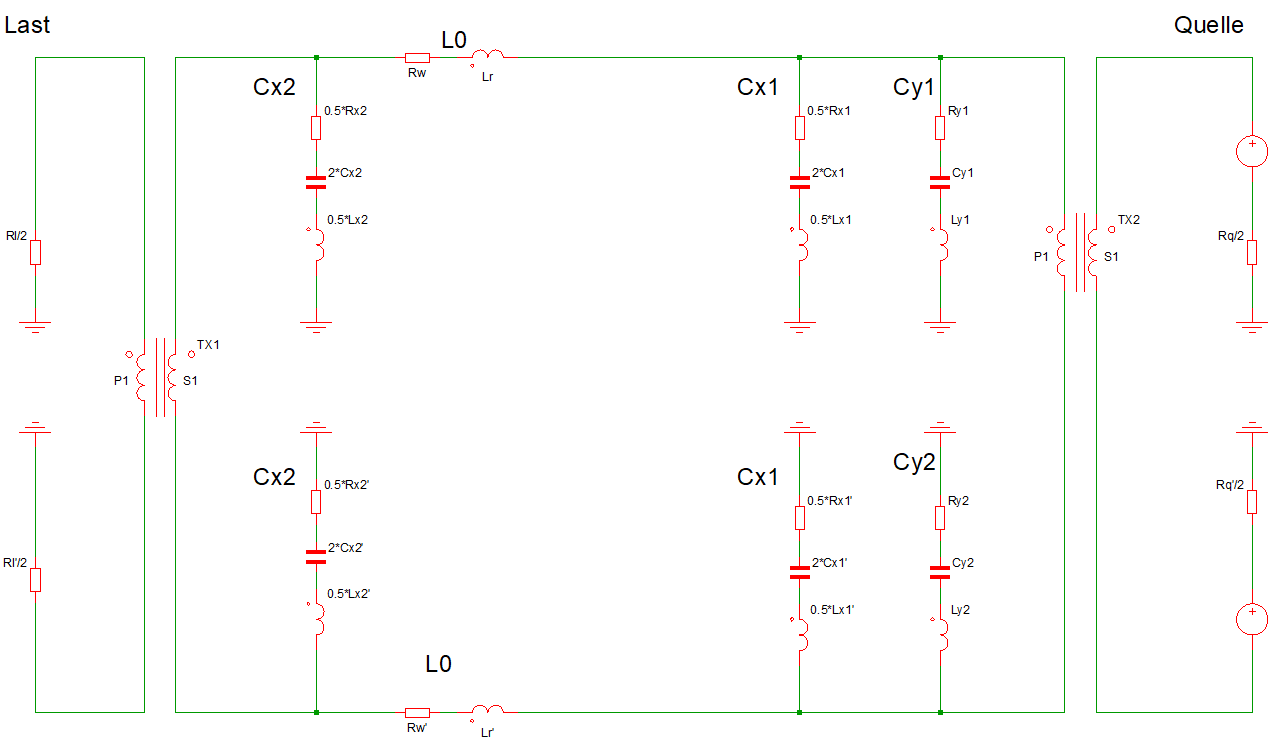
\includegraphics[width = 15cm]{EMI_DMpretty7.png}
	\caption{symmetrisch aufgetrennte Gegentaktschaltung}
	\label{fig:DMSchaltungSymAufgetrennt}
\end{figure}
Der obere und untere Teil der aufgetrennten Schaltung sind weitgehend identisch. Somit reduziert sich die Schaltung auf einen der beiden Stränge. Abbildung \ref{fig:DMSchaltungvereinfacht} zeigt die komplett vereinfachte Schaltung, welche die Grundlagen für die Gegentaktberechnungen bildet. 
\begin{figure}[H]
	\centering
	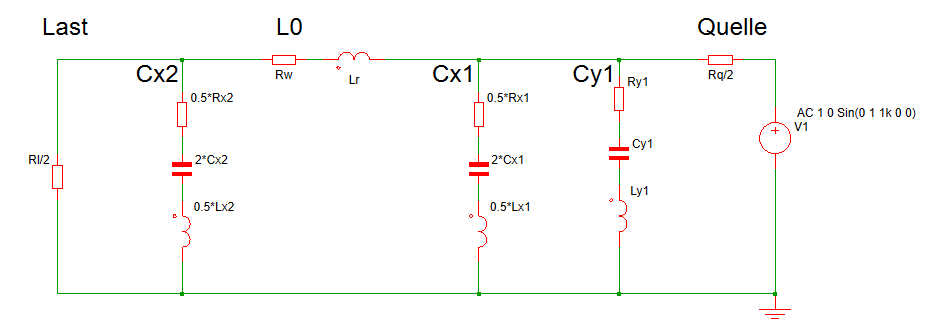
\includegraphics[width = 15cm]{EMI_DMvereinfacht.png}
	\caption{komplett vereinfachte Gegentaktschaltung}
	\label{fig:DMSchaltungvereinfacht}
\end{figure}

\paragraph{Bilden der Kettenmatrix}\label{para:kettenGegentakt}
Abbildung \ref{fig:dmschaltungEingeteilt} zeigt die Einteilung der reduzierten Schaltung in Längs- und Querimpedanzen.
 
\begin{figure}[H]
		\centering
		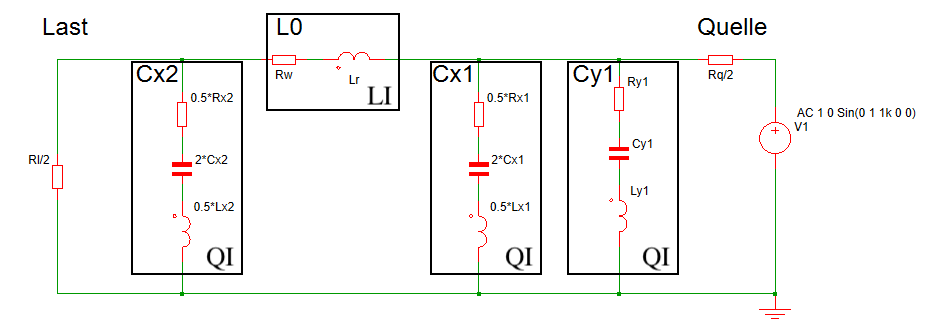
\includegraphics[width = 15cm]{EMI_DMvereinfacht_markiert.png}
		\label{fig:dmschaltungEingeteilt}
		\caption{Einteilung der Gegentaktschaltungsteile}
\end{figure}

Im nächsten Schritt werden die Impedanzen der einzelnen Schaltungsteile gebildet, welche in die passenden Kettenmatrizen eingesetzt werden.
Wiederum durch Kaskadierung der einzelenen Kettenmatrizen wird die Kettenmatrix der Gesamtschaltung gebildet. Aus der Kettenmatrix wird, wie bei der Gleichtaktschaltung die Einfügungsdämpfung berechnet.


